\documentclass[12pt]{article}
\usepackage{amsmath}
\usepackage[lmargin = 1in, rmargin = 1in, tmargin = 1in, bmargin = 1in]{geometry}
\usepackage[none]{hyphenat}
\usepackage{graphicx}
\usepackage{subcaption}
\usepackage{float}

\title{\textbf{Problem 4(b)}}
\author{Aditya Vipradas\\ASU ID: 1209435588}
\begin{document}
\maketitle
The gradient descent and Newton's methods are employed to find the minimum of the given convex function. Both the methods are complemented with the Armijo line search with t = 0.1, b = 0.55. The methods are tested for two guess values. Let us assume the first guess value to be [-1, 2]. The gradient descent with Armijo line search takes 64 iterations to arrive at the minimum for $x_{2}$ and $x_{3}$ as (-0.14289, 0.78573) whereas the Newton's method completes the search in 1 iteration as shown below and gives the minimum at (-0.14286, 0.78571). The epsilon i.e. gradient norm criterion is kept at 1e-4.
\begin{figure}[H]
\begin{center}
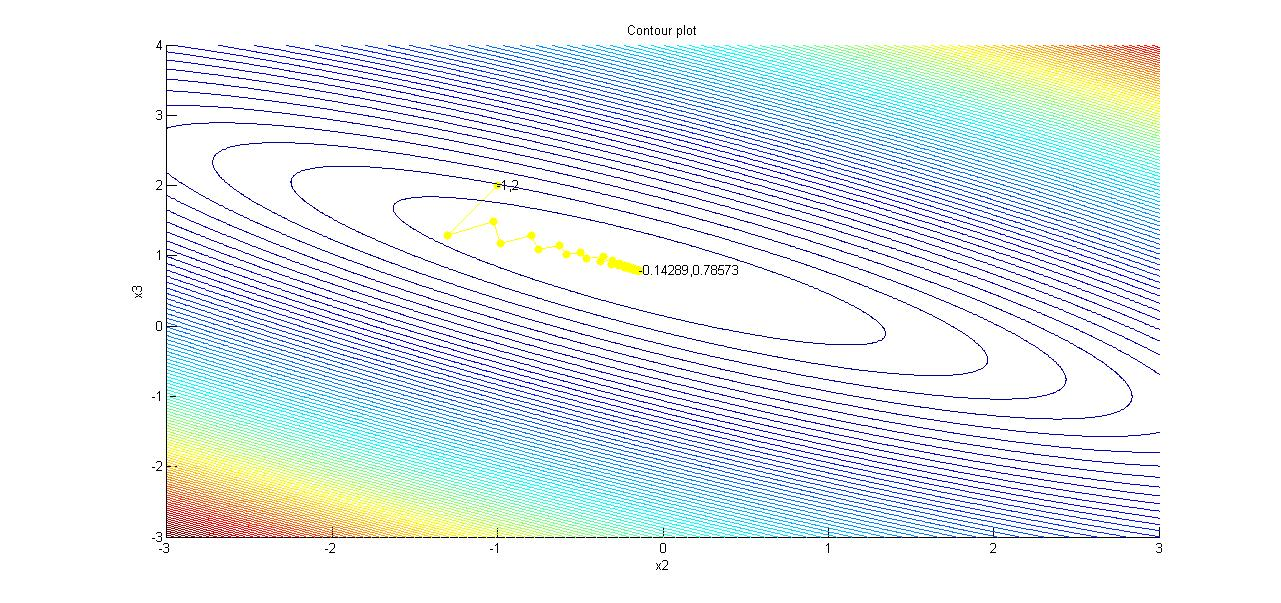
\includegraphics[scale=0.375]{contour2g.jpg}
\caption{Gradient descent with Armijo search for guess [-1, 2]}  
\end{center}
\end{figure}
\begin{figure}[H]
\begin{center}
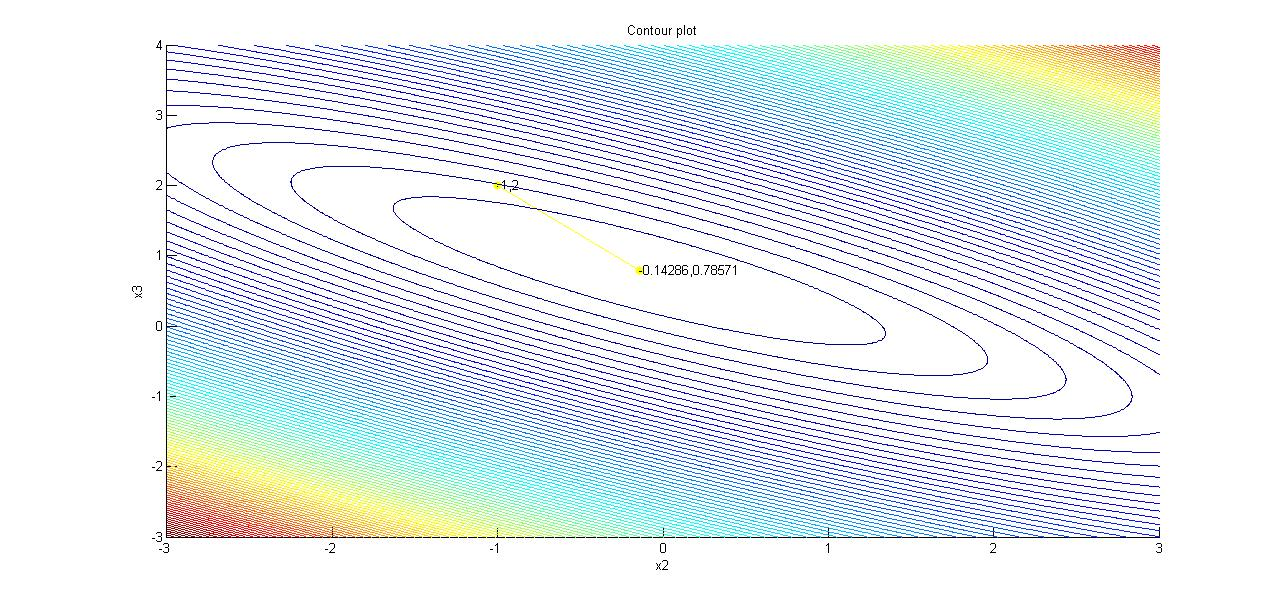
\includegraphics[scale=0.375]{contour2n.jpg}
\caption{Newton's method with Armijo search for guess [-1, 2]}  
\end{center}
\end{figure}
\begin{figure}[H]
\begin{center}
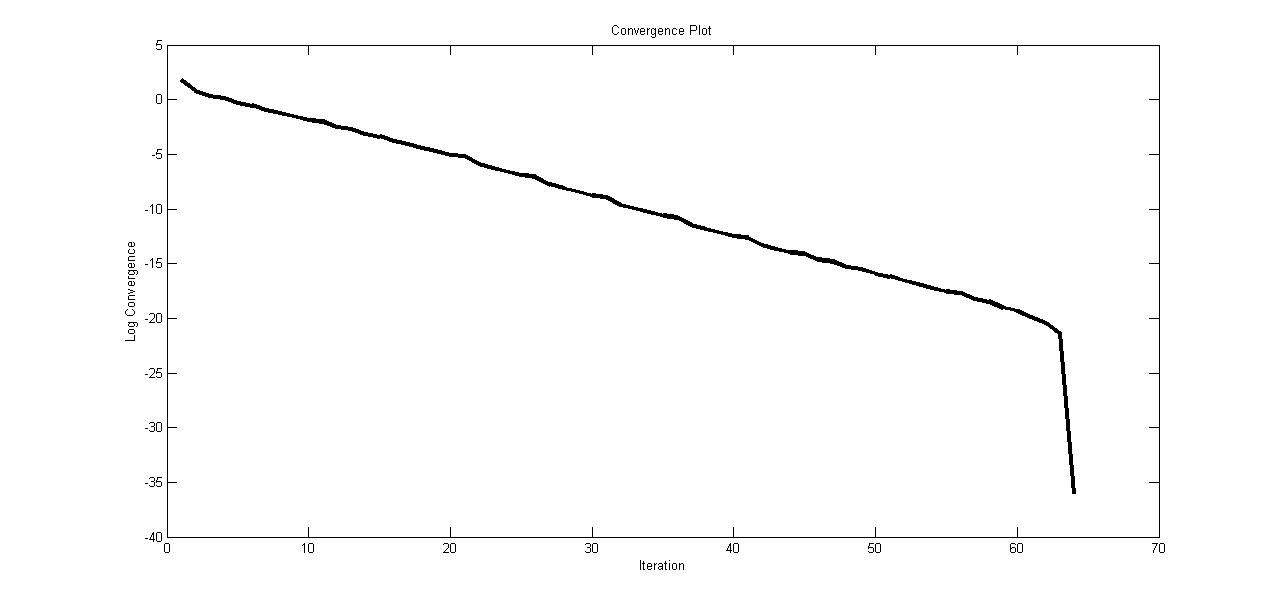
\includegraphics[scale=0.375]{conv2g.jpg}
\caption{Gradient descent convergence for guess [-1, 2]}  
\end{center}
\end{figure}
\begin{figure}[H]
\begin{center}
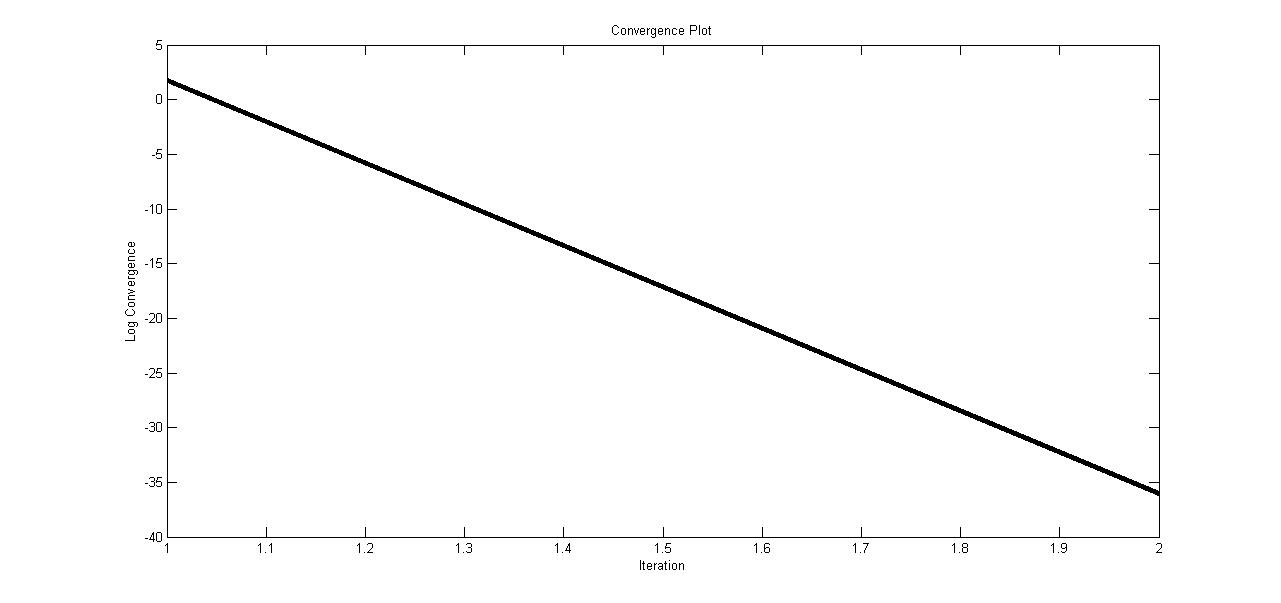
\includegraphics[scale=0.375]{conv2n.jpg}
\caption{Newton's method convergence for guess [-1, 2]}  
\end{center}
\end{figure}

The second guess value considered is [2, 3]. The gradient descent with Armijo line search takes 59 iterations to arrive at the minimum for $x_{2}$ and $x_{3}$ as (-0.14283, 0.7857) whereas the Newton's method completes the search in 1 iteration as shown below and gives the minimum at (-0.14286, 0.78571). The epsilon i.e. gradient norm criterion is kept at 1e-4.
\begin{figure}[H]
\begin{center}
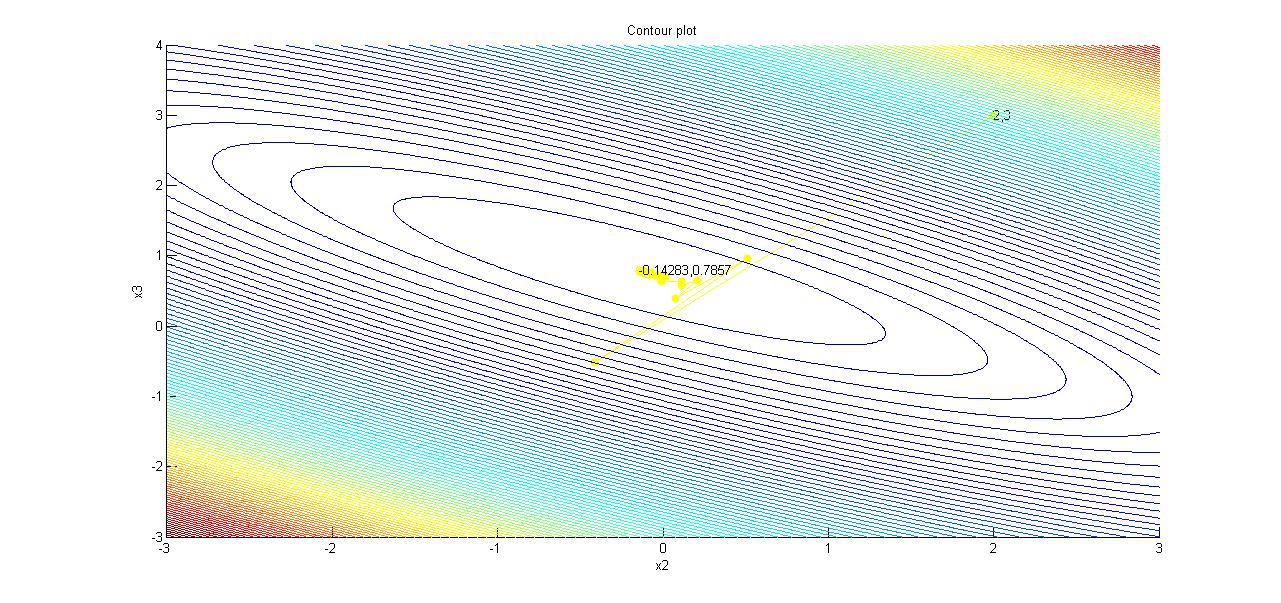
\includegraphics[scale=0.375]{contour1g.jpg}
\caption{Gradient descent with Armijo search for guess [2, 3]}  
\end{center}
\end{figure}
\begin{figure}[H]
\begin{center}
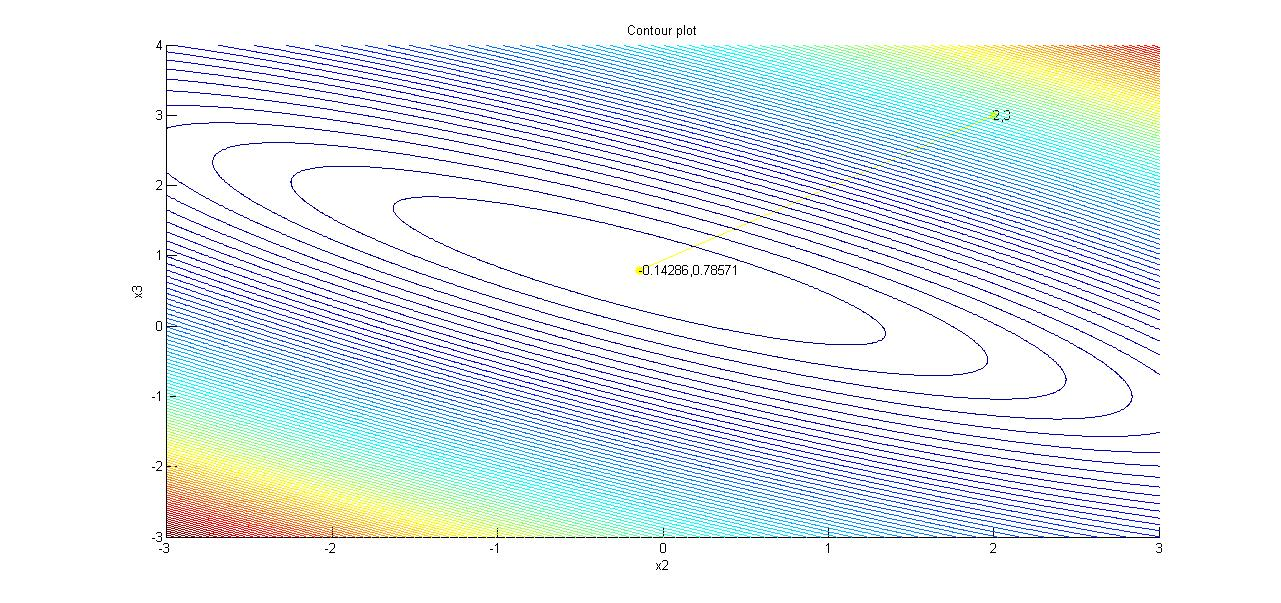
\includegraphics[scale=0.375]{contour1n.jpg}
\caption{Newton's method with Armijo search for guess [2, 3]}  
\end{center}
\end{figure}
\begin{figure}[H]
\begin{center}
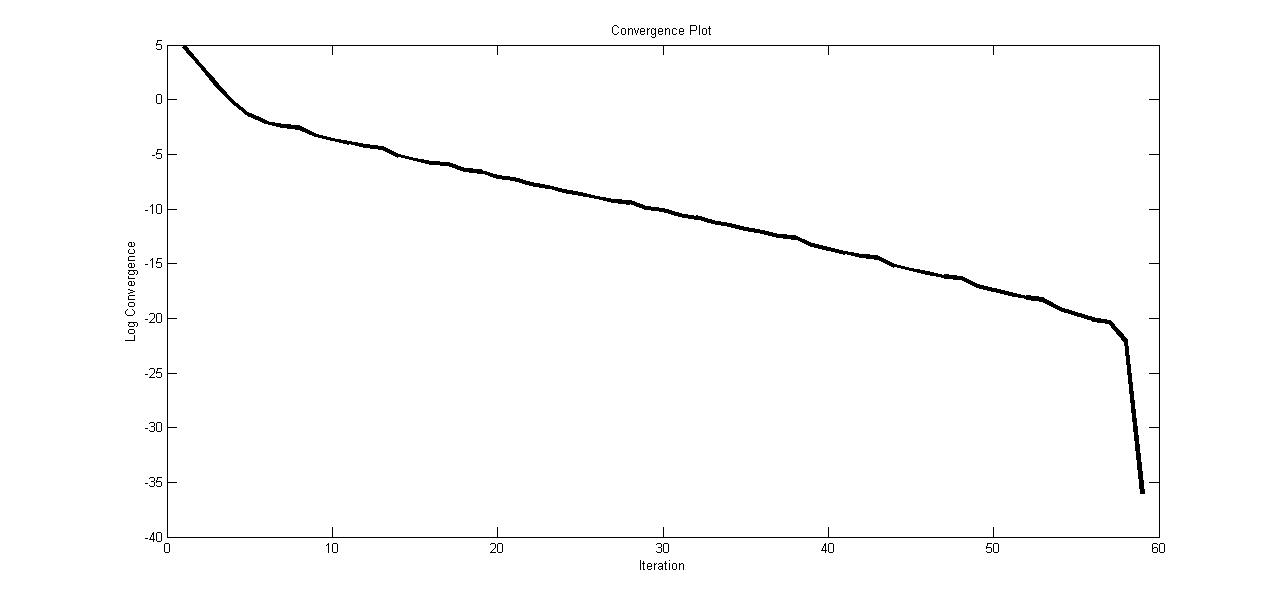
\includegraphics[scale=0.375]{conv1g.jpg}
\caption{Gradient descent convergence for guess [2, 3]}  
\end{center}
\end{figure}
\begin{figure}[H]
\begin{center}
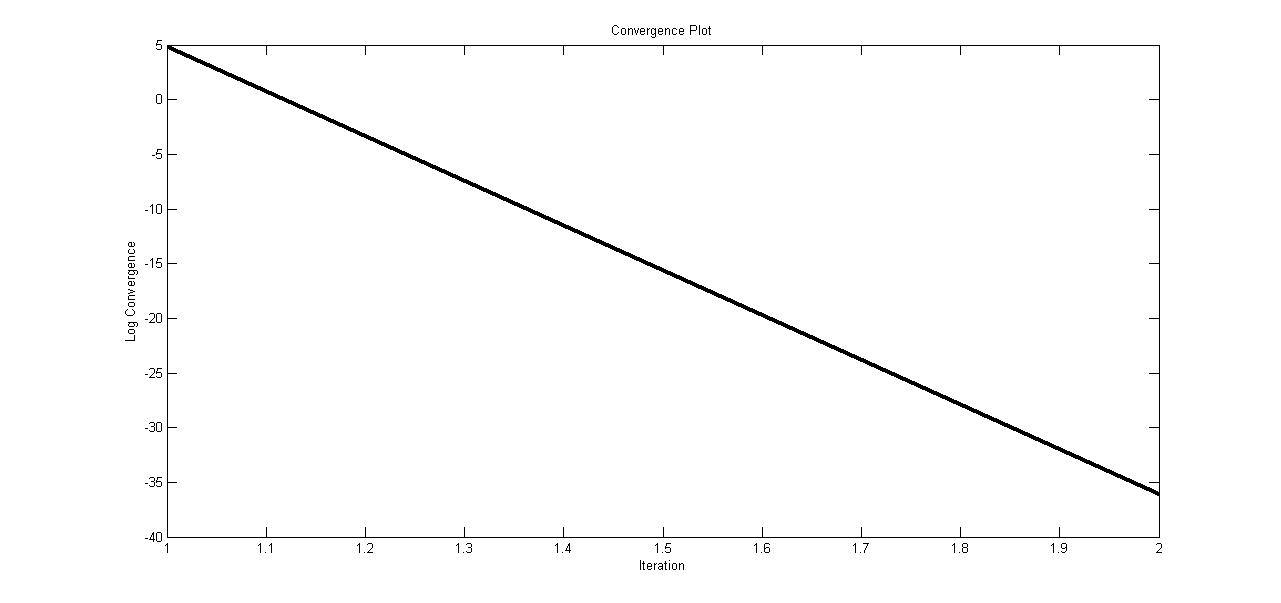
\includegraphics[scale=0.375]{conv1n.jpg}
\caption{Newton's method convergence for guess [2, 3]}  
\end{center}
\end{figure}
As observed from all the convergence plots, a log convergence between -35 and -40 is obtained which is acceptable. The plots for gradient descent is non-linear whereas it is linear for the Newton's method.
 
As seen from all the plots, the gradient descent method takes more number of iterations than the Newton's method to reach the minimum. The Armijo search method is employed in both the methods. Therefore, for the given problem, the Newton's method with Armijo line search is better because it tracks the global minimum in just one iteration. This is because the given objective function is quadratic and Newton's method approximates a given function as quadratic through Taylor's expansion. Hence, for a given quadratic convex function, the Newton's method can track the global minimum in a single step. (Find all the MATLAB codes in the following slides). 
\end{document}